%*****************************************************************************************************            
%                               INSTITUT MINES-TELECOM, IMT ATlantique
%                         Département Mathematical & Electrical Engineering           
%                                     Technopôle de Brest-Iroise                   
%                                  CS 83818 - 29238 BREST Cedex 3                       
%            
%                                    **  Tous droits réservés **
%                                      
%
% NOM DU PROJET : TP LaTeX 006 / Modèle de rapport de recherche (validé par la DRI), de support de cours
% et de TP au format LaTeX avec les éléments de la charte graphique de la communication d'IMT Atlantique
%
% LIVRABLE : [ ] Memo, [ ] Résumé, [ ] Article, [ ] Code, [X] Rapport , [ ] Thèse, [ ] Cours/TP
%
% AUTEUR(s) : Thierry LE GALL (Dépt. MEE), Guillaume ANSEL (SC), Thomas GUILMENT (Dépt. SC)
%
% HISTORIQUE :
%
% Date          Nom(s)          Version  Description
% ------------  --------------- -------  ----------------------------------------------------------
% 12-mar-2015   T. LE GALL (SC) 0.0      création du document 
% 26-mar-2016   T. LE GALL (SC) 0.1      mise à jour : essai du package UTF8
% 26-sep-2016   G. ANSEL        0.2      mise à jour : ajout exemple utilisation TBannexe
%                                        ajout correction titres en majuscule dans sommaire
%                                        (cf BUGFIX_TITRES_SOMMAIRE dans imta.sty)
%                                        changement polices utilisées
% 09-jan 2017   T. LE GALL (SC) 0.3      mise à jour : évolution du modèle de TB vers IMT Atlantique
% 03-fev 2017   G. ANSEL        0.4      mise à jour : modifications pour adaptation à version 1.5 du package imta
%                                        ajout méta-données PDF
% 14-fev-2017   T. GUILMENT     0.5      mise à jour : ajout package fancyhdr pour entêtes et pieds de page
%                                        changement style titres
% 16-fev-2017   G. ANSEL        0.6      mise à jour : modifications pour version 1.6 package imta
%                                        ajout style de page IMTAfancy pour entêtes et pieds de page
%                                        remplacement \listoffigures et \listoftables par \IMTAlistefigures
%                                        et \IMTAlistetableaux
% 17-fev-2017   G. ANSEL        0.7      mise à jour : déplacement définition style IMTAfancy dans imta.sty
%                                        définition commande \IMTAfooter pour personnaliser le pied de page
%                                        en bas à gauche
% 21-fev-2017   T. LE GALL (SC) 0.8      mise à jour : ajout d'un exemple de n° de contrat de recherche
%                                        (pied de page) et vérification de la compilation du document 
% 28-fev-2017   G. ANSEL        0.9      mise à jour : ajout exemple d'utilisation de l'option copyright
%                                        du package imta (informations copyright sur quatrième de couverture)
% 06-fev-2017   T. LE GALL (SC) 1.0      mise à jour : ajout de définitions d'ensembles mathématiques et exemple
%                                        d'édition de bloc dans le texte.  Ajout de la mention FIN DE FICHIER. 
%                                        Test de compilation avec imta.sty (v2.3) = PASS (0 errors, 0 warnings).
% 06-avr-2017   T. LE GALL (SC) 1.1      mise à jour : ajout du type de document et du numéro de rapport
%                                        de recherche en tant que paramètre du document et affichage des
%                                        informations en première de couverture (suite à demande de la DRI)
% 03-aoû-2017   T. LE GALL (SC) 1.2      mise à jour : exemple de section de texte sur deux colonnes et équations
%                                        dans deux blocs adjacents de style Beamer
% 09-aoû-2017   T. LE GALL (SC) 1.3      mise à jour : ajout des équations (matrices, vecteurs)
% 11-sep-2017   T. LE GALL (SC) 1.4      mise à jour : attribution du n°ISSN 2556-5060 pour les rapports de recherche
% 22-sep-2017   G. ANSEL        1.5      mise à jour : ajout d'un exemple d'insertion de tableau
% 25-sep-2017   T. LE GALL      1.6      mise à jour : légende du tableau et n° de version du modèle en page de garde
%                                        + tests de non-négression du modèle (env. Win 7) suite à BUGFIX_21092017_1
%                                         et BUGFIX_21092017_2 dans le fichier imta.sty v2.8 et v2.9
% 27-nov-2018   G. ANSEL        1.7      mise à jour : modifications pour passage en version 3.5 du package imta
% 21-jan-2019   T. LE GALL (SC) 1.8      mise à jour : couverture : type de document au-dessus de titre et liste
%                                        des auteurs et contributeurs sous le titre + tests de compilation (Win10)
%                                        + tests de compilation (UBUNTU 18.04 LTS)
% 10-mai-2020  T. LE GALL (SC)  1.9      mise à jour : ajout d'exemples supplémentaires (équations) 
% 25-jan-2021  T. LE GALL (MEE) 2.0      mise à jour : département Mathematical & Electrical Engineering                                      
%
%
% NOTES/COMMENTAIRES :
%
% - Exemple de rapport scientifique au format IMT Atlantique sous LaTex avec insertion de formules,
%   figures, ref. biblio, hyperliens, signets, renvois actifs, surlignage des formules. Le fichier
%   d'édition tp_latex_006.tex utilise le fichier de style imta.sty. Cf. fichier lab_006_readme.txt
%   situé sous le répertoire lab_006.
%
% REFERENCES :
%
% - cf. bibliographie
% 
%***********************************************************************************************

%-----------------------------------------------------------------------------------------------
%                                    DEBUT DU FICHIER D'EDITION
%-----------------------------------------------------------------------------------------------

\documentclass[11pt,a4paper,french]{article}

\usepackage{babel}
\usepackage[utf8]{inputenc}
\usepackage[T1]{fontenc}

\usepackage{newtxtext} % Police pour texte
\usepackage{newtxmath} % Police pour formules
\usepackage{textcomp}
\usepackage{graphicx}
\usepackage{amsmath}
\usepackage{microtype}

\usepackage{framed}	% Permet de surligner les résultats importants

% Charte graphique de IMT Atlantique
% L'option "version" affiche la menion "Document version x" sur la première de couverture
% Le numéro de version est paramétrable via la commande "\version"
% L'option "copyright" affiche la mention "© IMT Atlantique ..." sur la quatrième de couverture
% Les informations de copyright sont paramétrables via les commandes \IMTAanneecopyright, \IMTAdepotlegal, \IMTAissn

\usepackage[copyright]{../sty/imta} % édition avec copyright (et n°ISSN) en 4eme de couverture
%\usepackage{../sty/imta}	% édition sans copyright (et n°ISSN) en 4eme de couverture

% Signets et hyperliens (à charger en dernier)
\usepackage[colorlinks=true,linkcolor=black,urlcolor=blue,citecolor=IMTAbleu]{hyperref} 

%----------------- Métadonnées du PDF (facilite le travail des moteurs de recherche) -----------
\hypersetup{
	pdfinfo = {
		Author = {<Auteur 1>; <Auteur 2>; ...},
		Title = {<Titre du document>},
		Keywords = {<Mot-clé 1>; <Mot-clé 2>; ...}
	}
}

%--------------------------- Définition du contenu du pied de page ----------------------------

% Le pied de page contient par défaut le titre du document.
% Il peut être remplacé en décommentant l'une des lignes ci-dessous

%\IMTAfooter{Modèle de document \LaTeX{} IMT Atlantique} % Exemple de remplacement par un autre texte
\IMTAfooter{\thereportnumber} % Utilisation du numéro de rapport de recherche

%-------------------- Informations de copyright pour quatrième de couverture ------------------
%          (uniquement si l'option "copyright" est présente pour le package imta)

% Les lignes ci-dessous permettent de remplacer manuellement le mois et l'année
% d'édition pour le dépot légal si nécessaire. Par défaut, le mois et l'année
% courants lors de la compilation du document sont utilisés

\IMTAanneecopyright{2021}
\IMTAdepotlegal{Septembre 2017}

%-------------------------------------- Do not modify -----------------------------------------
																									
% le numéro ISSN est communiqué par la BNF à la DRI. N°fixé par la BNF en
% fonction du type de document. Ne concerne que la collection des rapports
% de recherche (et pas les autres types de document utilisant ce modèle).
\IMTAissn{2556-5060}

%----------------------------------- End of do not modify -------------------------------------

%----------------- Définitions d'ensembles et d'opérateurs mathématiques ----------------------

\def\Cset{\mathbb{C}} % complexes
\def\Hset{\mathbb{H}} % hilbert
\def\Nset{\mathbb{N}} % entiers naturels
\def\Qset{\mathbb{Q}} % rationnels
\def\Rset{\mathbb{R}} % reels
\def\Zset{\mathbb{Z}} % entiers relatifs
\def\Dset{\mathbb{D}} % disque unite ouvert
\def\Eset{\mathbb{E}} % esperance mathematique

%-------------------------------------- FIN DES DEFINITIONS ----------------------------------

\begin{document}

%---------------------------------------------------------------------------------------------
%                                   PAGE DE TITRE (please modify)
%---------------------------------------------------------------------------------------------

% Type de document
%\DocumentType{<Type de document>}  
\DocumentType{Collection des rapports de recherche d'IMT Atlantique}
%\DocumentType{Document support de BE et de TP}
%\DocumentType{Support de cours}
%\DocumentType{Support de TP}
%\DocumentType{Mémoire technique}


% Numéro de rapport de recherche (à remplacer)
% Commenter la ligne ci-dessous si le document n'est pas un rapport de recherche
\ReportNumber{N° rapport de recherche}


\entity{\textbf{\large{IMT Atlantique}}\\
% Dépt. Automatique productique et informatique\\
% Dépt. Électronique\\ 
% Dépt. Informatique\\ 
%Dépt. Image \& traitement de l'information\\
%Dépt. Langues \& culture internationale\\ 
%Dépt. Logique des usages, sciences sociales \& sciences de l'information\\ 
%Dépt. Micro-ondes\\ 
%Dépt. Optique\\
%Dépt. Physiques subatomiques et technologies\\
%Dépt. Sciences sociales et de gestion\\
Dépt. Mathematical \& Electrical Engineering\\
%Dépt. Systèmes énergétiques et environnement\\
%Dépt. Systèmes réseaux, cybersécurité et droit du numérique\\
Technopôle de Brest-Iroise - CS 83818\\
29238 Brest Cedex 3\\
Téléphone: +33 (0)2 29 00 13 04\\
Télécopie: +33 (0)2 29 00 10 12\\
%4, rue Alfred Kastler\\
%CS 20722\\
%44307 Nantes Cedex 3\\
%Téléphone: +33 (0)2 51 85 81 00\\
%Télécopie: +33 (0)2 99 12 70 08\\		
%2, rue de la Châtaigneraie\\
%CS 17607\\
%35576 Cesson Sévigné Cedex\\
%Téléphone: +33 (0)2 99 12 70 00\\
%Télécopie: +33 (0)2 51 85 81 99\\
%10, avenue Édouard Belin\\
%BP 44004\\
%31028 Toulouse Cedex 04\\
%Téléphone: +33 (0)5 61 33 83 65\\		
URL: \textbf{\href{http://www.imt-atlantique.fr/}{www.imt-atlantique.fr}}
}

%\docdescription{<Destinataire : >}

\title{<Titre du document>}
%\title{Étude d'une forme d'onde pour communications longues-distances par le canal acoustique sous-marin}

\author{
	Auteur 1\\Affiliation\and
	Auteur 2\\Affiliation\and
	Auteur 3\\Affiliation\and
	Auteur 4\\Affiliation\and
	Auteur 5\\Affiliation
}

\contributors{Contributeur 1, Contributeur 2...}

% Numéro de version du document, affiché sur la couverture
% Commenter cette ligne pour ne pas faire apparaître la version du document.
\version{2.0}

% Date d'édition du document
\date{\today}

%------------------------------------------ Do not modify ------------------------------------
\IMTAfrontcover
\pagestyle{IMTAfancy} % Changement du style de page pour avoir en-tête et pied de page
%--------------------------------------- End of do not modify --------------------------------

%% Affichage des listes et tables.
\IMTAsommaire
\newpage
\IMTAlistefigures  % commenter pour ne pas avoir la liste des figures
\IMTAlistetableaux   % commenter pour ne pas avoir la liste des tables
\newpage
%---------------------------------------------------------------------------------------------
%                                   INTRODUCTION (please modify)
%---------------------------------------------------------------------------------------------

\section{Introduction} % exemple de structure d'introduction d'après [Lichtfouse 2012]

D'après \cite{[Lichtfouse2012]}, la structure d'une introduction est composée des éléments suivants :
\begin{enumerate}
	\item l'explication du contexte d'étude ou de la problématique annoncés dans le résumé avec l'arrière
	      plan et les enjeux;
	\item l'annonce de ce qui est étudié et fait dans le contexte d'étude ou pour tenter de résoudre la
	      problématique abordée;
	\item l'annonce des différentes parties du document : « dans un premier temps nous étudions... », « dans
	un deuxième temps nous abordons... », etc.
\end{enumerate}

%---------------------------------------------------------------------------------------------
%                                   CORPS DU DOCUMENT (please modify)
%---------------------------------------------------------------------------------------------

\section{Études et expérimentations}\label{sec:S_EXP}

Exemple de note de bas de page : OFDM\footnote{Orthogonal Frequency Division Multiplexing}.

\subsection{Étude ou expérience 1}\label{sec:SS_EXP1}

Exemple d'édition d'équation :

\begin{equation}
\label{E_AA_OFDM_BB_TMD_RX3_FREQ4}
Y(f) = \frac{1}{\sqrt{T}}\sum_{p=0}^{P-1}\sum_{k=-\infty}^{+\infty}\sum_{n=0}^{N-1}\frac{1}{a_k^{(p)}}
       e^{-j 2\pi\frac{n}{T}\tau_0^{(p)}}e^{j\Phi_0^{(p)}}
			 e^{-j2\pi \frac{f}{a_k^{(p)}}(kT+\tau_0^{(p)})}
			 d_k^{(n)}G_e(\frac{f-f_{d,k}^{(p)}}{a_k^{(p)}}-\frac{n}{T}).
\end{equation}

Autre exemple d'édition d'équation :

\begin{equation}
\label{E_RX_DETECT_DP4}
\textup{E}\{|y_k^{(n,p)}|^2\} = \underbrace{\textup{E}\{|\gamma_{k}^{(0, p)}|^2\} \textup{E}\{|d_k^{(n)}|^2\}}_{signal}
+\underbrace{\sum_{\stackrel{n'=0}{n'\neq n}}^{N-1}\textup{E}\{|\gamma_{k}^{(n'-n, p)}|^2\} \textup{E}\{|d_{k}^{(n')}|^2\}
+\textup{E}\{|w_k^{(n,p)}|^2\}}_{bruit}.
\end{equation}

Exemple d'édition d'équation avec surlignage (mise en évidence d'un résultat) :

\definecolor{shadecolor}{gray}{0.95}
\begin{shaded}
\begin{equation}
\label{E_SIGN_RX_BB_FREQ}
Y(f) = \sum_{p=0}^{P-1}\frac{1}{a^{(p)}} e^{j\Phi_0^{(p)}}e^{-j2\pi \left(\frac{f-f_d^{(p)}}{a^{(p)}}\right)\tau_0^{(p)}}
X\left(\frac{f-f_d^{(p)}}{a^{(p)}}\right).
\end{equation}
\end{shaded}

Exemple d'édition d'une expression matricielle :

\begin{equation}
\mathbf{\Gamma_k^{(p)}} = 
\left(
\begin{array}{cccc}
	\gamma_{k}^{(0, p)} 		&\gamma_{k}^{(1, p)} 			&\ldots &\gamma_{k}^{(N-1, p)} \\
	\gamma_{k}^{(-1, p)}		&\gamma_{k}^{(0, p)} 			&\ldots &\vdots								 \\
	\vdots              		&\vdots              			&\ddots &\vdots                \\
	\gamma_{k}^{(-(N-1), p)}&\gamma_{k}^{(-(N-2), p)}	&\ldots &\gamma_{k}^{(0, p)}
\end{array}
\right).
\end{equation}

Exemple d'édition d'expression vectorielle :

\begin{equation}
\label{E_RX_DETECT_DP3M}
\mathbf{y_k^{(p)}} = e^{j\Phi_0^{(p)}}\big(\mathbf{\Gamma_k^{(p)}}\otimes \mathbf{\Phi^{(p)}}\big)\mathbf{d_k} + \mathbf{w_k^{(p)}},
\end{equation}

\begin{equation}
\label{E_RX_WK_VECT}
\mathbf{w_k^{(p)}} = [w_k^{(0,p)},...,w_k^{(n,p)},...,w_k^{(N-1,p)}]^T.
\end{equation}

Exemple d'écriture d'équations avec multiples valeurs possibles à droite :

\begin{equation}
\label{E_PULSE}
p_W(t)= 
\{
\begin{array}{cc}
A,  &-\frac{W}{2} \leq t \leq \frac{W}{2}\\
0,  &\text{otherwise}
\end{array}
\end{equation}

Exemple d'écriture d'équation sur plusieurs lignes avec alignement des termes (environnement \emph{aligned} du package \emph{amsmath}) :

\begin{equation}
\label{E_MOD_PULSE_FIN_TRAIN_SED}
\begin{aligned}
|S(f)|^2 = &(\frac{AWL}{\sqrt{2}T_r})^2sinc_{\pi}^2[(f-f_0)W]\\
&(\sum_{k=-\infty}^{+\infty}sinc_{\pi}[(f-f_0-\frac{k}{T_r})L])^2
\end{aligned}
\end{equation}

\newpage % exemple de saut de page
\subsection{Étude ou expérience 2}\label{sec:SS_EXP2}

Exemple de figure au format \texttt{*.png} (de préférence), possiblement \texttt{*.jpg} (Figure \ref{fig:F_STRUCT_TRAME_TX}):

\begin{figure}[htb]
\centering
%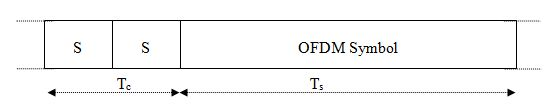
\includegraphics[width=10cm]{structure_trame_tx.jpg}
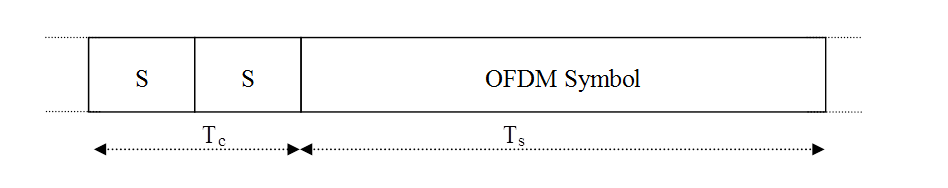
\includegraphics[width=14cm]{structure_trame_tx.png}
\caption{Structure de la trame à l'émission}\label{fig:F_STRUCT_TRAME_TX}
\end{figure}

\subsection{Étude ou expérience 3}\label{sec:SS_EXP3}

Exemple de définition éditée dans un bloc de style \emph{Beamer} :

\begin{beamerblock}{Définition}
$B=(B_t)_{t\in\Rset_+}$ \`a valeurs r\'eelles est un {\bf mouvement brownien} (ou {\bf processus de Wiener}) issu de $x$ si
\begin{enumerate} 
\item $B_0=x$ 
\item $0\leq t_i\leq t_j \Rightarrow B_{t_j}-B_{t_i}\sim \mathcal{N}(0,\sigma^2(t_j-t_i))$
\item $0\leq t_i\leq t_j\leq t_k\leq t_l \Rightarrow \Eset[(B_{t_j}-B_{t_i})(B_{t_l}-B_{t_k})]=0$
\end{enumerate}
\end{beamerblock}

~\\ %exemple de saut de ligne insécable
\indent
Exemple d'équations éditées dans 2 blocs adjacents de style \emph{Beamer} :

\begin{multicols}{2}
	
	\begin{beamerblock}{\centering{Coarse Cross-correlation}}
		\begin{equation}
		A_c^{(m)} = \sum_{i=0}^{N_c-1}u_k^{(m+i)}u_k^{*(m+i+N_c)}.
		\end{equation}
	\end{beamerblock}
	
	\begin{beamerblock}{\centering{Fine Cross-correlation}}
		\begin{equation}
		A_f^{(m)} = \sum_{i=0}^{N_c-1}u_k^{(m+i)}u_k^{*(m+i+N_{f\prime})}.
		\end{equation}
	\end{beamerblock}
	
\end{multicols}

\subsection{Étude ou expérience 4}\label{sec:SS_EXP4}

Exemple d'un texte édité sur deux colonnes adjacentes :

\begin{multicols}{2}
	Voici un exemple de texte édité sur 2 colonnes dans le modèle de document de rapport de recherche IMT Atlantique. Ce modèle
	est édité en langage \LaTeX{} adapté à la rédaction de documents scientifiques contenant, notamment, des équations et des figures.
\end{multicols}

\subsection{Étude ou expérience 5}\label{sec:SS_EXP5}

Exemple d'insertion de tableau :

\begin{table}[htb]
	\centering
	\begin{tabular}{lcc}
		\toprule
		\textbf{Nom}             & \textbf{Type} & \textbf{Nombre d'heures} \\ \midrule
		FIG MTS 203P (com. num.) &    Module     &            10            \\
		FIP RT323 (codage)       &    Module     &            10            \\
		FIP MGP320 (projet S5)   &      UV       &            15            \\
		FIG F4B301 (codage)      &      UV       &            20            \\ \bottomrule
	\end{tabular}
	\caption{Exemple de tableau (données factices)} \label{tab:T_ENSEIGNEMENT}
\end{table}

\section{Résultats}\label{sec:S_RES}

<Placer le texte ici>

\subsection{Résultat 1}\label{sec:SS_RES_1}

D'après \cite{[Lichtfouse2012]}, la structure d'une présentation de résultats est composée des éléments
suivants :
\begin{enumerate}
	\item description du résultat (ce qu'il faut observer);
	\item discussion du résultats (commenter les observations);
	\item conclusions sur le résultat (que peut-on en déduire ?).
\end{enumerate}

%---------------------------------------------------------------------------------------------
%                                   CONCLUSIONS (please modify)
%---------------------------------------------------------------------------------------------
\newpage
\section{Conclusions}

% Rappel des résultats majeurs
Résumer les résultats majeurs obtenus...

\begin{itemize}
	% Result 1
	\item Résultat 1 \ldots
	% Result 2
	\item Résultat 2 \ldots
	% Result 3
	\item Résultat 3 \ldots
\end{itemize}

% Interpretations
Exposer les interprétations...

% Conséquences, bénéfices et inconvénients
Tirer les conséquences, bénéfices ou inconvénients...

% Perspectives (travaux futures)
Dégager les perspectives ouvertes et/ou annoncer les futurs travaux (le cas échéant)...

%--------------------------------------- DEBUT DES ANNEXES --------------------------------------
\newpage
\begin{IMTAannexes}
	
%-------------------------------------------- ANNEXE 1  -----------------------------------------
	
\IMTAannexe{Exemple d'annexe}\label{sec:S_ANN_EX}

Un exemple d'annexe.
\section{Première partie}


\subsection{Sous-section}
\subsection{Sous-section}

\section{Deuxième partie}

\subsection{Sous-section}
\subsection{Sous-section}

%-------------------------------------------- ANNEXE 2  -----------------------------------------

\IMTAannexe{Autre annexe}\label{sec:S_ANN_EX2}

Un autre exemple d'annexe.
\section{Première partie}


\subsection{Sous-section}
\subsection{Sous-section}

\section{Deuxième partie}

\subsection{Sous-section}
\subsection{Sous-section}

%------------------------------------- -- FIN DES ANNEXES --------------------------------------
\end{IMTAannexes}

%-----------------------------------DEBUT DE LA BIBLIOGRAPHIE ----------------------------------
\newpage
%------------------ Ajout du renvoi vers la bibliographie dans le sommaire ---------------------
\phantomsection
\addcontentsline{toc}{section}{\refname}
%-----------------------------------------------------------------------------------------------

\begin{thebibliography}{99}
\bibitem{[Lichtfouse2012]} Eric Lichtfouse, \emph{Rédiger pour être publié}, Springer, $2^{eme}$ édition, 2012
 (cote bibliothèque IMT Atlantique Brest : $0.343$ LICH).
 
%----------------------------------- FIN DE LA BIBLIOGRAPHIE -----------------------------------
\end{thebibliography}
%---------------------------------------- Do not modify ----------------------------------------
\IMTAcoverpage
%------------------------------------ End of do not modify -------------------------------------

\end{document}

%***********************************************************************************************
%                                   FIN DU FICHIER D'EDITION
%***********************************************************************************************
